\section{Solutions}
Multiple solutions are introduced in this part, starting with a preliminary naive approach and then refining it step by step to arrive at a definitive solution. The idea is to start with one of the traditional methods for handling recommendation systems and then improve it by combining it with many data mining techniques designed for handling massive amounts of data. 

\subsection{Naive solution}
\label{naive_solution}
Building a recommendation system based on the traditional methodologies is the easiest and most straightforward way to address the aforementioned problem; as was covered in the section on related work, the two primary approaches for these kinds of tasks are content-based and collaborative filtering. Considering that the input of the problem is an utility matrix partially filled with ratings and the remaining cells left blank, the choice fell in a first stage on collaborative filtering rather then content based, avoiding in this way to define item and user profiles. The choice of collaborative filtering gives the possibility to build either an Item-Item or a User-User collaborative filtering recommendation system, where the missing values — the cells $U_{ij}$ in the utility matrix that are blank — are filled according to one of the following schema:
\begin{enumerate}
    \item Item-Item collaborative filtering: this technique looks for the top $K$ queries that are most similar to query $j$ in the utility matrix. The average of the top-K items as rated by user $i$ is then used to fill the value for $U_{ij}$.
    \item User-User collaborative filtering: This method is similar to the previous one in concept, but differs slightly in that instead of looking for the top-K items that are similar to item $j$, this method looks for the top-K users that are similar to user $i$, and the value $U_{ij}$ is then filled with the average of the K most similar users to user $j$ that have rated item $j$. 
\end{enumerate}

Both these strategies requires to define a similarity measure to locate a neighborhood of K similar items or users. Due to a number of factors, which can be summed up as follows, the Item-Item approach was chosen over the User-user approach: 
\begin{itemize}
    \item Item's neighbourhood tends to change much slower in comparison to user's neighborhood. This is due to the fact that the user-user approach is good at making recommendations to users with unique tastes;
    \item Explainability of the model. In comparison to describing why a person has similar preferences to another, it is considerably simpler to explain the reasoning behind why an item has been recommended to a certain user based on previously rated goods; 
    \item Finding items of the same type is easier than finding users who only like items of a particular type, so item-item similarity frequently provides more reliable information;
    \item The systems considered in the aforementioned problem definition typically have more users than items, and the more users there are, the more expensive it will be to find the K closest neighbors. 
\end{itemize}

\subsubsection{Choosing a similarity measure}
\label{choosing_a_similarity_measure}
Finding a good similarity measure is crucial for making a solid neighborhood choice, but there are a few factors to take into account before choosing the best one. Two similarity measures — the Jaccard similarity and the Cosine similarity — were introduced in the section \ref{similatrity_measures} on similarity measures, one for sets (including binary vectors) and the other for vectors in euclidean space.
The optimal similarity measure for this problem is the Cosine similarity, considering that neighborhood selection is based on item ratings corresponding to a column of the utility matrix i.e. a vector.
Even though the Jaccard similarity is not appropriate for handling vectors, a slightly modified version of this similarity measure is provided in the section for the next solution in order to handle vectors of user ratings. 

% pseudocode
\subsubsection{Pseudocode} The idea of Item-Item collaborative filtering is to iterate over all the utility matrix's cells. If a cell $U_{ij}$ is empty, it's rating is predicted by averaging the ratings of user $i$ for the $K$ queries that are most similar to query $j$. The similarity between two queries is given by the \emph{cos\_sim} procedure which takes as input two vectors to compare; the vector of the ratings of all the users for a single query $j$ is denoted as $U_{*j}$. In the pseudocode the neighborhood size $K$ is assumed to be $1$, i.e. the rating for $U_{ij}$ is predicted with the rating of user $i$ in the query that is most similar to query $j$.

\begin{algorithm}[h]
	\caption{Naive version of Item-Item collaborative filtering} 
	\begin{algorithmic}[1]
	    \For{$i \gets 1$ to $|S|$}  
	        \For{$j \gets 1$ to $|Q|$}
	            \If{$U_{ij} = \varnothing$} \Comment{Find empty cells $U_{ij}$}
	                \For{$q \gets 1$ to $|Q|$}  
        	            \State $\text{sim} \gets \text{sim} \cup \text{cos\_sim}(U_{*j}, U_{*q})$
                    \EndFor
                    \State $top \gets \argmax \,sim$ \Comment{Find most similar query}
                    \State $U_{ij} \gets top_i$
	            \EndIf
            \EndFor
        \EndFor
	\end{algorithmic} 
\end{algorithm}

This method involves computing the cosine similarity for each potential pair of queries. The cost of computing the cosine similarity is equal to the cost of computing the dot product of two queries, each of which corresponds to a column vector of $|S|$ components and has a cost of $O(|S|)$. The final cost to predict one single missing value of the utility matrix is given by $O(|S|\cdot|Q|^2)$. It's clear that predicting all the missing values of the utility matrix is costly, in particular when the dealing with a massive amount of users and queries.

\subsection{MinHash for LSH}
\label{minhash_section}
The primary issue with the previous solution is the algorithm's time complexity. In particular, the cost of finding the top $K$ queries that are similar to a given query is largely driven by the need for the algorithm to compute the similarity between all potential combinations of queries in the utility matrix. In order to address this issue, a more effective technique is presented in this section that employs minHash\cite{minhash} in conjunction with LSH to increase the similarity search's speed at the expense of accuracy. The purpose of LSH is to avoid checking the similarity between items that are definitely dissimilar and to concentrate solely on pairs of items that are likely to be similar; the latter are referred as \emph{candidate pairs}. Finding those candidate pairs in the original utility matrix is expensive; for this reason the idea is to apply LSH on a signature matrix rather than on the original utility matrix.

\subsubsection{MinHash} LSH typically operates on small signatures derived from a \emph{characteristic matrix}, which is a common representation of the data in order to describe the characteristic of the items. In the specific case of documents, the characteristic may be seen as a matrix $C$ with each row representing a potential word from a given vocabulary and each column representing a document: the word $i$ is present in the document $j$ if and only if $C_{ij} \neq 0$. There is a clear connection between the concept of characteristics matrix and the concept of utility matrix of recommendation systems, with the latter being a characteristics matrix in which each column $j$ is an item(a query) and each row $i$ corresponds to a user: the user $i$ has rated item $i$ if and only if $C_{ij} \neq 0$. This correlation between the twos clearly allows to exploit the MinHash technique to obtain a compressed representation of the utility matrix(from now on the utility matrix is considered to be the characteristic matrix). 

Dealing with the utility matrix directly is impractical in some cases due to its massive size; for this reason the idea is to replace the characteristics matrix with a compressed version called \emph{signature matrix} in such a way that the similarity of the items in the signature matrix is as close as possible to the similarity of items in the original characteristics matrix. No method can guarantee that the similarity will be exactly the same because some information from the characteristics matrix may be lost despite the fact that it was crucial in determining the similarity. The MinHash technique\cite{minhash} has been devised for the Jaccard similarity, thus as more signatures are added to the signatures matrix, the estimate of the Jaccard similarity between two items will get more accurate and similar to that for the original utility matrix.

The idea of MinHash is to generate a signature matrix $\delta$ by taking a number of $H$ of permutations $\pi$ of the rows of the utility matrix $U$(corresponding to the characteristics matrix) and finding for each of the items the first row in the permutation $\pi_t$ of $U_{*j}$ that has a value of one, i.e.
\begin{equation}
\begin{aligned}
\delta_{tj} \gets \text{min}_\pi (U_{\pi_tj} = 1)
\end{aligned}
\end{equation}



\paragraph{Example} Given a utility matrix $U$ of three items and a set of two permutations $\pi$, the signature matrix $\delta$ is produced as follows. 

\vspace{1em}
\begin{minipage}{0.3\linewidth}
    \centering
    $\pi=$
    \begin{tabular}{|l|l|l|}
    \hline
        \textbf{$\boldsymbol \pi_1$} & \textbf{$\boldsymbol \pi_2$} \\ \hline
        4 & 6 \\ \hline
        3 & 3 \\ \hline
        6 & 4 \\ \hline
        2 & 1 \\ \hline
        1 & 5 \\ \hline
        5 & 2 \\ \hline
    \end{tabular}
\end{minipage}
\begin{minipage}{0.3\linewidth}
    \centering
    $U=$
    \begin{tabular}{|l|l|l|}
    \hline
        \textbf{$\boldsymbol i_1$} & \textbf{$\boldsymbol i_2$} & \textbf{$\boldsymbol i_3$} \\ \hline
        1 & 1 & 1 \\ \hline
        0 & 1 & 1 \\ \hline
        1 & 0 & 0 \\ \hline
        0 & 0 & 0 \\ \hline
        0 & 1 & 1 \\ \hline
        1 & 0 & 1 \\ \hline
    \end{tabular}
\end{minipage}
\begin{minipage}{0.3\linewidth}
    \centering
    $\delta = $
    \begin{tabular}{|l|l|l|}
    \hline
        \textbf{$\boldsymbol i_1$} & \textbf{$\boldsymbol i_2$} & \textbf{$\boldsymbol i_3$} \\ \hline
        4 & 1 & 1 \\ \hline
        1 & 3 & 2 \\ \hline
    \end{tabular}
\end{minipage}


\subsubsection{Permutations generation} Generating the permutations and storing them in memory might be infeasible when dealing with utility matrices having a massive amount of users. For this reason a possibility is to simulate the effect of random perturbations by picking $H$ hash functions, one for each permutation, that return the index of a given row in the permutation. 

\begin{equation}
\begin{aligned}
\pi(x) = (ax + b) \bmod c
\end{aligned}
\end{equation}

where $a$, $b$ and $c$ are random value less than the number or users in the utility matrix, i.e $a, b, c \leq |S|$.

\subsubsection{Adapted MinHash for ratings} Given that the Jaccard similarity is defined for sets and consequently binary vector as exposed in Section \ref{similarity_measure_jaccard}, there is a problem in the above formulation of MinHash because it assumes that the characteristics matrix is made of 0s and 1s. However in the problem formulation, described in Section \ref{problem_statement}, the utility matrix $U$ is made of ratings in the range $[1,100]$. A solution for this problem is to convert the utility matrix $U$ containing the ratings into a matrix $\widehat{U}$ of zeros and ones, where the value $\widehat{U}_{ij} = 1$ indicates that the user $i$ has liked query $j$. Given that the threshold at which a query might be considered liked or not might vary depending on the situation, a threshold parameter named $T$ is introduced, according to which a query is considered liked if its rating is greater than $T$, i.e. 
\begin{equation}
\begin{aligned}
\widehat{U}_{ij} = 1 \iff U_{ij} \geq T
\end{aligned}
\label{eq_ratings}
\end{equation}
 
\paragraph{Example} Given a utility matrix $U$ of ratings in the range $[1,100]$, missing ratings denoted by cells with a value of $0$, and a threshold level of $T=50$ above which a rating is deemed to be positive, the corresponding utility matrix $\widehat{U}$ of positive ratings is obtained according to Eq. \ref{eq_ratings} as shown below. 

\vspace{1em}
\begin{minipage}{0.5\linewidth}
    \centering
    $U=$
    \begin{tabular}{|l|l|l|}
    \hline
        \textbf{$\boldsymbol q_1$} & \textbf{$\boldsymbol q_2$} & \textbf{$\boldsymbol q_3$} \\ \hline
        80 & 5 & 12 \\ \hline
        0 & 67 & 0 \\ \hline
        46 & 85 & 0 \\ \hline
        0 & 55 & 65 \\ \hline
        35 & 10 & 90 \\ \hline
        95 & 0 & 45 \\ \hline
    \end{tabular}
\end{minipage}
\begin{minipage}{0.5\linewidth}
    $\widehat{U}=$
    \begin{tabular}{|l|l|l|}
    \hline
        \textbf{$\boldsymbol q_1$} & \textbf{$\boldsymbol q_2$} & \textbf{$\boldsymbol q_3$} \\ \hline
        1 & 0 & 0 \\ \hline
        0 & 1 & 0 \\ \hline
        0 & 1 & 0 \\ \hline
        0 & 1 & 1 \\ \hline
        0 & 0 & 1 \\ \hline
        1 & 0 & 0 \\ \hline
    \end{tabular}
\end{minipage}

\vspace{1em}

The computation of the modified version of the utility matrix in practice is computationally expensive, in particular given $|S|$ and $|Q|$ respectively the number of users and the number of queries in the utility matrix, the cost of making such conversion is $O(|S| \cdot |Q|)$, which is quadratic in the size of the input. To overcome this issue a possibility is to use a slightly modified version of MinHash, denoted as \emph{MinHash with threshold}, that assigns to the signature matrix entry $\delta_{tj}$ the index of the first row in the permutation with a rating above the threshold level $T$.

\begin{equation}
\begin{aligned}
\delta_{tj} \gets \text{min}_\pi (U_{\pi_tj} \geq T)
\end{aligned}
\end{equation}

The resulting signature matrix is a good approximation for a modified version of the Jaccard similarity measure in order to take into account positive ratings as $1$ if they are greater than a threshold $T$ and $0$ the elements that are smaller than $T$. 

An implementation of this idea in pseudocode is shown in Algorithm \ref{minhash_alg}. The idea is to iterate over all queries and $H$ permutations of the utility matrix rows to discover the first row in the permuted order of the utility matrix that has a rating higher than the threshold $T$. In most cases, the loop of line 4 requires less iterations then the total number of users $|S|$ in the utility matrix.
The index $i$ is used as an input to create the permuted index $u$, increasing by one with each iteration until it reaches a maximum value of $|S|$. 

\begin{algorithm}[h]
    \caption{MinHash algorithm: signature matrix generation} 
    \begin{algorithmic}[1]
        \For{$j \gets 1$ to $|Q|$}
            \For{$h \gets 1$ to $H$}   
                \State $i \gets 1$ \Comment{$i$ is the original index of the rows}
                \While{$\delta_{hj} = \varnothing \cap i \leq |S|$} 
                    \State $u \gets \pi_h(i)$ \Comment{$u$ is the permutation of row $i$}
                    \If{$U_{uj} \geq T$} 
                        \State $\delta_{hj} \gets i$
                    \EndIf
                    \State $i \gets i + 1$
                \EndWhile
            \EndFor
        \EndFor
    \end{algorithmic} 
    \label{minhash_alg}
\end{algorithm}

\subsubsection{Locality Sensitive Hashing} \label{lsh_description}
Once the signature matrix has been generated according to the modified version of MinHash with threshold $T$, the following step is to use the Locality Sensitive Hashing(LSH) technique to hash the queries in the signature matrix several times, in such a way that similar queries, i.e. queries with similar ratings, are more likely to be hashed to the same bucket than dissimilar queries are. The signature matrix is divided into $b$ bands, each made up of $r$ rows. Each band is then column-wise hashed into a set of buckets that is specific to that band, and queries that hashed to the same bucket are then considered to be candidate pairs. The information included in the candidate pairs can be used to reduce the time required to detect similar queries, so that each query $i$ is tested for similarity with each query $j$ that lie in the same bucket as query $i$ for at least one band, i.e. query $i$ and query $j$ are candidate pairs. 

The number of bands $b$ and the number of rows for each band $r$ play a crucial role in the amount of candidate pairs found for each query. In fact these two parameter are directly related one with the other i.e. recalling that $H$ is the number of permutation, namely the number of rows of the signature matrix $\delta$ then it holds that $b \cdot r = H$. Given this connection, it follows that the number of candidate pairs that LSH will find will increase if there are many bands and, as a result, few rows per band. On the other hand, if there are few bands and a large number of rows per band, LSH will locate fewer items that are similar to each other. A good trade-off must be chosen for the parameter $b$ defining the number of bands or equivalently for the parameter $r$ defining the number of rows for each band: the size of the signature matrix and the distribution of the data in the original utility matrix are two important criteria that must be taken into consideration while choosing these parameters; in the latter scenario, it is possible that all of the queries are extremely dissimilar from each other, which means that even a small value of $r$ is able to capture a significant number of candidate pairs. In the opposite scenario, it's possible that every query is incredibly similar to each other query, indicating that a low value of $r$ is insufficient and that the number of rows per band should be increased to prevent an excessive number of similar items from going against the goal of finding a good compromise on the number of similar items. 



\subsubsection{Making recommendations} \label{making_rec}
The final step is to provide recommendations using the item-item collaborative filtering method, similar to the one used in the Naive solution, with the exception that in this case, the iterative process that identifies the queries with the highest degree of similarity only iterates on the candidate pairs of a given query rather than on all possible queries. Considering time complexity, in the worst scenario the number of candidate pairs identified for each query is equal to the set of all the queries, leading the algorithm to fall back on the naive method. However this is just a limit case, in fact the number of candidate pairs can be reduced by appropriately adjusting the number of bands $b$ and the number of permutations $H$. 


\subsection{SimHash for LSH}
\label{simhash_section}
The Jaccard similarity, used with MinHash, is not the proper similarity measure for the problem taken into consideration; in fact, as discussed in section \ref{choosing_a_similarity_measure}, the Jaccard similarity is not the optimal similarity measure for vectors. In some situations, the modified version of the Jaccard similarity that takes the threshold parameter $T$ into account fails to measure the similarity between two queries. This situation occurs, for instance, when two queries have a rating that is remarkably similar, such as $49$ and $51$, but the threshold parameter $T=50$ makes them different. This problem is brought on by the indirect conversion of the utility matrix into a matrix of zeros and ones indicating whether a user liked or didn't like a query. A more suitable similarity measure for the problem under consideration in this study is the Cosine similarity, which can be computed on vectors of any type rather than only binary vectors.

This algorithm's general structure is quite similar to the one discussed for the solution with MinHash for LSH. The goal of the algorithm is to create a signature matrix $\delta$ that is representative of the original utility matrix, which means that given two general queries, their similarity should be preserved as much as possible in the signature matrix. The computation of the signature matrix should be quick and affordable, allowing the algorithm to benefit from using the signature matrix rather than the original utility matrix. After computing the signature matrix, the following step is to apply LSH to it in order to identify local similarities used to generated a set of candidate similar queries.


\subsubsection{SimHash intuition} The intuition behind of SimHash is to generate a signature matrix of $H$ rows, dividing the space containing the vectors corresponding to queries into $H$ hyperplanes passing through the origin. For any given hyperplane, each query ends up in one region of the hyperplane, either above or below the hyperplane. The signature matrix is filled for each query with its position with respect to the hyperplane $H_i$ corresponding to one row of the signature matrix $\delta$. The idea is that the closer two queries are, the more probable it is that they will be on the same region for a random hyperplane. For instance, on the majority of the planes that can be randomly generated, two queries that are relatively close to each other will end up in the same region.  The example in Figure \ref{fig:random_planes} accurately illustrates the intuition by demonstrating that for any arbitrary number of random hyperplanes and two similar queries $\vec{q_1}$ and $\vec{q_2}$, the probability of the queries falling on different sides of the hyperplanes is relatively small compared to the total number of hyperplanes: in that specific case, only the red plane divides the two queries into two different sides of the plane. SimHash has been demonstrated to be a locality-sensitive hash function that roughly approximates the cosine similarity\cite{simhash_demonstration} \cite{simhash_demonstration2}. 


\begin{figure}[h]
\begin{tikzpicture}[line cap=round,line join=round,>=triangle 45,x=1cm,y=1cm]
\begin{axis}[
    width=0.45*\textwidth,
    height=6.5cm,
    axis lines=middle,
    xmin=-10,
    xmax=10,
    ymin=-10,
    ymax=10,
    xtick={-10,-8,...,10},
    ytick={-10,-8,...,10},
    yticklabels={,,},
    xticklabels={,,}]
    
    \draw [-stealth, line width=1pt] (0,0) -- (6,8);
    \draw [-stealth, line width=1pt] (0,0) -- (8,6);
    \draw [line width=1pt,color=gray,domain=-100:100, dashed](-10,-2.776524) -- (10, 2.776524);
    \draw [line width=1pt,color=gray,domain=-100:100, dashed](-2.776524,-10) -- (2.776524, 10);
    \draw [line width=1pt,color=red,domain=-100:100, dashed](-10,-10) -- (10, 10);    
    \draw [line width=1pt,color=gray,domain=-100:100, dashed](-10,10) -- (10, -10);    
    \draw [line width=1pt,color=gray,domain=-100:100, dashed](2.776524,-10) -- (-2.776524, 10);
    \draw [line width=1pt,color=gray,domain=-100:100, dashed](-10, 2.776524) -- (10, -2.776524);

    \begin{scriptsize}
    \draw[color=black] (6,9) node {$\vec{q_1}$};
    \draw[color=black] (9,6) node {$\vec{q_2}$};
    \end{scriptsize}
\end{axis}
\end{tikzpicture}
\caption{\normalfont Two similar queries $\vec{q_1}$ and $\vec{q_2}$ are more likely to fall into the same region of any random hyperplane than when they are dissimilar.} 
\label{fig:random_planes}
\end{figure}

\subsubsection{Signature matrix computation} 
The computation of the signature matrix is straightforward based on the prior intuition: generate $H$ random hyperplanes and fill the ith row of the signature matrix with the query's position relative to the hyperplane. From a more formal perspective an \emph{hyperplane} is represented in a n-dimensional space with an n-dimensional vector that is orthogonal to the hyperplane. The position of a query vector $\vec{q_j}$ with respect to a general hyperplane $H_t$, represented by its orthogonal vector $\vec{h_t}$, is given by the sign of the projection of $\vec{q_j}$ on $\vec{h_t}$. Given that the projection of a vector on another one is computed using the dot product, the signature matrix cell corresponding to the ith hyperplane represented by its orthogonal vector $\vec{h_t}$ and the jth query $\vec{q_j}$ is computed as follows

\begin{equation}
\begin{aligned}
\delta_{tj} \gets \sign(\vec{h_t} \cdot \vec{q_j})
\end{aligned}
\end{equation}

where the $\sign$ function returns a value of $1$ if the argument that it takes as input is positive, otherwise it returns $-1$. The values of $1$ and $-1$, respectively, indicate that the query vector is located either on the positive or negative side of the hyperplane.
\begin{equation}
  \sign(\vec{h_t} \cdot \vec{q_j})=\begin{cases}
    1 & \text{if $\vec{h_t} \cdot \vec{q_j} \geq 0$}.\\
    0 & \text{otherwise}.
  \end{cases}
\label{sign_func}
\end{equation}

\paragraph{Example} Consider the example depicted in Figure \ref{fig:projection} of a generic hyperplane $H_1$ represented by its orthogonal vector $\vec{h_1} \in \mathbb{R}^2$ and two queries $\vec{q_1},\vec{q_2} \in \mathbb{R}^2$, characterized by the ratings given by two users. The position of the queries with respect to the hyperplane is determined by projecting $\vec{q_1}$ and $\vec{q_2}$ onto $\vec{h_1}$ and checking the sign, i.e. computing the sign of the dot product between the two vectors. In this specific instance, both queries are found to be on the positive side of the hyperplane $H_1$, therefore the corresponding cell in the signature matrix is filled with a value of $1$. Following the notation of signature matrix cell $\delta_{ij}$, defining the $ith$ row(the $ith$ hyperplane) and the $jth$ column(the $jth$ query) of the signature matrix, the signature for the first plane $H_1$ and the aforementioned queries is filled with $\delta_{11} \gets 1$ and $\delta_{12} \gets 1$.

\begin{figure}[h]
\begin{tikzpicture}[line cap=round,line join=round,>=triangle 45,x=1cm,y=1cm]
\begin{axis}[
    width=0.45*\textwidth,
    height=6.5cm,
    axis lines=middle,
    xmin=-42,
    xmax=45,
    ymin=-15,
    ymax=45,
    xtick={-40,-30,...,50},
    ytick={-10,0,...,50}]
    \clip(-41.94512591313005,-13.436694591890513) rectangle (57.578131814683154,49.31752666468061);
    \draw [-stealth, line width=1pt] (0,0) -- (30,25);
    \draw [-stealth, line width=1pt] (0,0) -- (10,40);
    \draw [line width=1.5pt,color=gray,domain=-100:100, dashed] plot(\x,{(-0--3.163372054762762*\x)/8.446133593990732});
    \draw [-stealth,color=gray, line width=1.5pt] (0,0) -- (-14.983685711606949,40.006110270862);
    \draw [mark=none, gray,thick, dotted] (-4.52,12.07)-- (30,25);
    \draw [mark=none, gray,thick, dotted] (-11.91,31.79)-- (10,40);
    \begin{scriptsize}
    \draw[color=black] (13,42) node {$\vec{q_1}$};
    \draw[color=black] (33,27) node {$\vec{q_2}$};
    \draw[color=black] (-12,20) node {$\vec{h_1}$};
    \draw[color=black] (-35,-9) node {$H_1$};
    \end{scriptsize}
\end{axis}
\end{tikzpicture}
\caption{\normalfont Projection of queries $\vec{q_1}$ and $\vec{q_2}$ onto $\vec{h_1}$ to find their position with respect to the hyperplane $H_1$.} 
\label{fig:projection}
\end{figure}




%% reprocessing, normalize the space 
\paragraph{Preprocessing} Given that a query in the utility matrix is represented by a vector of positive ratings with values between 1 and 100, all query vectors will always be located in the positive quadrant of the space. In the 2-dimensional example depicted in Figure \ref{fig:projection}, all the queries will always be located in the upper rightmost quadrant. This behavior is problematic because, regardless of the query, the projection on any hyperplane defined by an orthogonal vector falling within the aforementioned quadrant will always have a positive sign. To overcome this issue the solution is to normalize the utility matrix's ratings into the range $[-50,50]$ by subtracting the average value of $50$ from all the ratings in the utility matrix that are not $0$(missing rating), i.e. the new utility matrix $\widehat{U}$ is computed as follows:
\begin{equation}
\begin{aligned}
\widehat{U}_{ij} \gets U_{ij} - 50   && \forall i,j  \text{ s.t. } U_{ij} \neq 0
\end{aligned}
\end{equation}

The initial utility matrix $U$ is shown on the left in the example of Figure \ref{fig:standardization}, and the new utility matrix $\widehat{U}$, which is centered in $0$, is shown on the right. 



\begin{figure}[h]
    \begin{minipage}{0.49\linewidth}
        \centering
        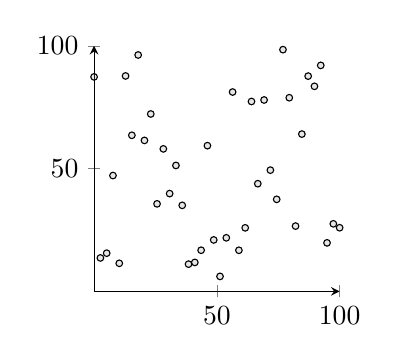
\begin{tikzpicture}
        \begin{axis}[
                axis lines=middle,
                height=4.7cm, width=4.7cm,
                xmin=0,
                xmax=100,
                ymin=0,
                ymax=100,
                xtick={0,50,...,100},
                ytick={0,50,...,100}
                ]
            \pgfmathsetseed{7}%
            \addplot+[y filter/.expression={y},only marks,mark=*,draw=black, mark size=1.2pt, mark options={fill=gray},fill opacity=0.2,samples=40,domain=-0:100] {100*rnd};
        \end{axis}
        \end{tikzpicture}
    \end{minipage}
    \begin{minipage}{0.49\linewidth}
        \centering
        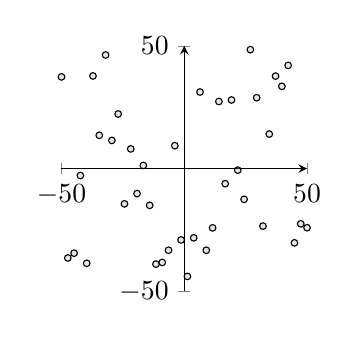
\begin{tikzpicture}
        \begin{axis}[
                axis lines=middle,
                height=4.7cm, width=4.7cm,
                xmin=-50,
                xmax=50,
                ymin=-50,
                ymax=50,
                xtick={-50,0,...,50},
                ytick={-50,0,...,50}
                ]
            \pgfmathsetseed{7}%
            \addplot+[y filter/.expression={y-50},only marks,mark=*,draw=black, mark size=1.2pt, mark options={fill=gray},fill opacity=0.2,samples=40,domain=-50:50] {100*rnd};
        \end{axis}
        \end{tikzpicture}
    \end{minipage}
    \caption{\normalfont The rating of the queries that originally are in the range $[1,100]$ are centered in the space to obtain ratings in $[-50,50]$.} 
    \label{fig:standardization}
\end{figure}


\paragraph{Pseudocode} Compared to the MinHash-based approach for producing the signature matrix, the SimHash algorithm is significantly simpler. Assuming that $H$ is a set of $|H|$ randomly generated hyperplanes, $\widehat{U}$ is the pre-processed utility matrix and $\sign$ is the function defined by Equation \ref{sign_func}, the signature matrix is computed as follows


\begin{algorithm}[h]
    \caption{SimHash algorithm: signature matrix generation} 
    \begin{algorithmic}[1]
        \For{$j \gets 1$ to $|Q|$}
            \For{$t \gets 1$ to $|H|$}   
                \State $\delta_{tj} \gets \sign(\widehat{U}_{*j} \cdot \vec{h_t})$
            \EndFor
        \EndFor
    \end{algorithmic} 
    \label{simhash_alg}
\end{algorithm}

\subsubsection{Making recommendations} Similar to the approach with MinHash, the next step is to leverage the signature matrix's information to find local similarities between queries using the Locality Sensitive Hashing technique outlined in Section \ref{lsh_description}. Given that not all candidate pairs correspond to similar queries, the candidate pairs need to be manually checked for similarity. According to the item-item collaborative filtering approach discussed in Section \ref{making_rec}, similar queries can be used to generate recommendations. The idea is to predict the rating of users $i$ to query $j$, which corresponds to $U_{ij}$ in the utility matrix, as the average of the ratings given by user $i$ for the $K$ queries that are most similar to query $j$. The complete architecture is shown in the diagram of Figure \ref{fig:cf_lsh}.
\begin{figure}[H]
    \centering
    \includegraphics[width=0.43\textwidth]{imgs/cf_lsh_diagram.pdf}
    \caption{\normalfont Architecture of the collaborative filtering recommendation system using LSH to quickly identify related queries.}
    \label{fig:cf_lsh}
\end{figure}

\subsection{Content based recommendations}  \label{hybrid_rec_sys_solution}
Given that the similarity of queries is related to both their properties as well as their ratings given by users, it is possible for users to give the same ratings to two queries even when they are completely different. In light of this, the previous method — which combines collaborative filtering and LSH — is ineffective for providing relevant suggestions since it only took into account the ratings of queries rather than their structure.
Consequently, the idea is to combine the algorithm considered in the previous sections(LSH in combination with collaborative filtering) with a content-based strategy, to build an hybrid recommendation system. This new approach takes advantage of both the properties of the queries as well as the ratings given by the users to provide pertinent query recommendations based on previous user activity. The properties of a query can be interpreted from a conceptual or from a results-oriented point of view, respectively a query can be seen as a conjunction of conditions or as a collection of tuples. 

\subsubsection{Item and user profiles} Content-based recommendation systems look through item properties to find items that a specific user may be particularly interested in. This kind of recommendation system works on the principle of creating user and item profiles, one for each system user and one for each item, respectively. The principle is that after the profiles are created, it should be easy to calculate how much a user could appreciate an item: compare the user profile to that of the item, and if a high similarity is found, it is probable that the user would appreciate that item. 

\paragraph{Query profiles} An item profile should describe the important features of an item, for example in the case of movies, it might be the actors that are part of the movie. According to the same logic, the characteristics of a query, as previously noted, can be represented by its conditions or by the set of tuples it returns. In the instance examined in this work, the decision fell to take into account item profiles (referred to \emph{query profiles} throughout this paper) as the tuples returned by each query. The query profile for a generic query $j$, denoted as $IP_j$, is represented as vector with the same number of components as the total number of rows of the relational table. The $ith$ component of $IP_j$ is set $1$ if the query $j$ returned the $ith$ row of the relational table, otherwise $0$. For example the query profile of a generic query $j$ that returns only the first and the third row of a relational table with 5 rows can be represented as $IP_j = [1,0,1,0,0]$. 

\paragraph{User profiles} User profiles describe the user preference to the features of items profiles, for this reason to compare user profiles with query profiles, user profiles must have the same number of components of item profiles. Since each component of the user profile correspond to a row of the relational table, the issue becomes evident: In the utility matrix, the user's preferences are expressed on queries rather than the rows that the queries return, so it's not clear how to express the user preference of a single row. To solve this problem the solution is to find the rows returned by each query(simulating a DBMS) and then compute the preference of user $t$ to the $ith$ row of the relational table as the average rating given by user $t$ to all the queries returning the $ith$ row of the relational table. Throughout the article, the user profile for user $t$ is referred to as $UP_t$. 


\subsubsection{Hybrid recommendation system} 
Once user and query profiles have been appropriately generated, they can be used to match users with potentially interesting items. The approach is to calculate the Cosine similarity between all the the vectorized user and item profiles in order to predict how much the user would likely appreciate an item. As already discussed in Section \ref{cosine_similarity} the cosine similarity measures the angle between two vector, so if the cosine similarity between an item profile $IP_j$ and a user profile $UP_t$ is high, it means that the angle between the two vectors is small, thus the user $t$ will probably like the query $j$. % However finding the potential matches between user profiles and query profiles involves computing the similarity between all the possible combinations of them, which is computationally expensive.
The idea, which is accurately depicted in Figure \ref{fig:hybrid}, is to build an \emph{Hybrid recommendation system} that combines the content-based approach introduced in this section with the collaborative filtering technique mentioned in the earlier solutions: the algorithm uses at first collaborative filtering with LSH to find the $K$ most similar queries of each query based on the user ratings in the utility matrix, then on top of that, the algorithm exploits content-based information derived from the queries to generate more accurate recommendations. As shown in figure \ref{fig:hybrid} the content-based phase attempts to match each user of the system with the optimal query among the $K$ most similar queries found by collaborative filtering: each user's profile is compared to the profile of each query among the $K$ that are most similar to a particular one. 

Similarly to the previous method, this one begins by running LSH with collaborative filtering. However, instead of predicting the missing ratings using the average of the $K$ most similar queries, it then runs content based to determine which query will be the best match for the user. 


\begin{figure}[h]
    \centering
    \includegraphics[width=0.43\textwidth]{imgs/hybrid_diagram.pdf}
    \caption{\normalfont Architecture of the hybrid recommendation system}
    \label{fig:hybrid}
\end{figure}




\subsection{Measuring the importance of a query(Part B)}

The aforementioned algorithm has been making recommendations based on queries that were already part of the query set, meaning that at least one user had submitted them. It's clear that in a more advanced scenario, queries that have not yet been posed to the DBMS might be of interest to the users of the system. Based on this, the purpose of this section is to provide a method for determining the importance of a query in general for all the users, i.e. how much the users of the system would like a query that may or may not have already been asked to the DBMS. 

Measuring the importance of a query must be done carefully and taking into account all the information that is available in the current system. For this reason there are several resources that can be helpful to build a system that computes the importance of a query; First of all there are two fundamental inputs:
\begin{itemize}
    \item the utility matrix filled with the missing ratings $(U)$
    \item the query itself, defined as a set of conditions $(q)$
\end{itemize}

The two aforementioned are the main inputs, but there are also some indirect inputs as a result of the utility matrix being calculated utilizing some other resources, namely the relational table $(R)$ and the query set $(Q)$. 

\begin{definition}[Importance]
For the purposes of this research, the \emph{importance} of a query has been defined in a way to assigns an integer value that is high if users in general will find that specific query interesting or a low value if users may think it is not significant at all. It was decided to use the convention of quantifying the importance of a query on a percentage scale that ranges from 0\% (not relevant) to 100\% (important).
\end{definition}


There are numerous approaches to finding a simple importance metric that could guarantee a precise enough measurement, but most of the time these approaches only use information from the relational table without considering the user's ratings, which is not enough when the objective is to deliver a sophisticated method that accurately measures the importance. The solution proposed in this section takes into account both the preferences of the users, expressed in terms of the utility matrix, and the factual utility of a query obtained by the rows that it returns from the relational table. Consequently, the suggested algorithm is divided into a preprocessing phase followed by two important steps: the first step computes the importance of a query based on the user ratings provided in the utility matrix, whereas the second one leverages the rows returned by the query, i.e. the result of a query.

\subsubsection{Preprocessing}
This early phase runs the query through the DBMS and produces results that allow some queries that could initially be considered as unimportant to be excluded from the subsequent phases. The idea is that queries returning all of the rows from the relational table $R$ or queries returning nothing at all should be treated as unimportant, and the algorithm should therefore assign them a low relevance rating, let's say $0\%$. This task usually takes very little time and is crucial because a query's outputs serve as its primary measure. 
This step is useful as generally a user would judge a query as a good one if it returns at least some outcomes, but not all the results. If the query is not labelled as unimportant in this preprocessing phase, the algorithm moves on with the next step.
\begin{algorithm}[h]
    \caption{Preprocessing} 
    \begin{algorithmic}[1]
        \State $rows \gets executeQuery(q)$
        \If{$rows = \varnothing$ or $rows = R$}
            \State $importance \gets 0\%$
        \Else
            \State $Step1()$
        \EndIf
    \end{algorithmic} 
    \label{alg:PartB_Preprocessing}
\end{algorithm}


\subsubsection{Step 1}

This step takes into consideration users' preferences provided by the utility matrix. The idea in this phase is to first obtain the average rating of each query from the utility matrix, by taking the average of each single column, corresponding to a query, and then compute the average rating given to each feature $f_i$ of that query as the average rating given by users to queries containing that feature $f_i$. In detail, as soon as each query $q_i$ is splitted into its conditions, the next step is to gather all of the features that shape each condition, without considering the value of that condition(recall that a feature is a relational table column, for example considering the condition $f_1 = Trento $ then $f_1$ is the feature and $Trento$ is the value). As each feature  $f_i$ is gathered, the algorithm gives to each feature $f_i$ a value of importance that is proportional to the average rating given by users to queries containing feature $f_i$. If a feature has no recorded grade, it will be counted as non important, so it will be assigned a 1\% grade. 

\paragraph{Example} Consider a feature \emph{city} which appears in only two queries of the query set, namely $q_1$ and $q_2$; suppose that according to the utility matrix the average ratings of query $q_1$ and $q_2$ are respectively $70$ and $90$. The average grade to the \emph{city} feature is computed as the average of $70$ and $90$, that is $80$.


\vspace{1em}
Once all the feature ratings are retrieved, the partial query importance(result of this first part) is computed as the average of its features' importance. To get this outcome the idea is to use the Geometric Mean\cite{geometric_mean} as the average measure of importance. The choice to use the Geometric Mean is driven by the necessity to give more emphasis to low rated features rather than highly rated features: given that a query is defined as a conjunction of condition, all the conditions must be satisfied in order for the query to return a specific row, thus even a negative grade on a single feature probably means that the entire query is not useful at all. 
The Algorithm \ref{alg:PartB_Step1} illustrates the pseudocode defining the process of computing the first partial importance, where the partial calculation of a query's importance computed in this first step is indicated as $I_a$. 

\begin{algorithm}[h]
    \caption{Step 1} 
    \begin{algorithmic}[1]
        \State $queryScore \gets []$
        \For{$j \gets 1$ to $|Q|$}\Comment{Avg rating of each query in Q}
            \State $queryScore_i \gets avg(U_{*j})$
        \EndFor
        \State
        \State $featureRating \gets []$
        \For{$f_i $ in $R.features$} \Comment{Avg rating of each feature in R}
            \State $featureScore \gets []$
            \For{$j \gets 1 $ to $ |Q|$}
                \If{$f_i$ in $q_j$}
                    \State $featureScore \gets featureScore \cup queryScore_j$
                \EndIf
            \EndFor
            \State $featureRating_{f_i} \gets avg(featureScore)$
        \EndFor 
        \State
        \State $queryFeatures \gets []$
        \For{$f_i $ in $R.features$} \Comment{Importance of the query q}
            \If{$f_i$ in $q$}
                \State $queryFeatures \gets queryFeatures \cup featureRating_{f_i}$
            \EndIf
        \EndFor
        \State $I_a \gets GeoMean(queryFeatures)$
    
    \end{algorithmic} 
    \label{alg:PartB_Step1}
\end{algorithm}


\subsubsection{Step 2}
In the previous step the importance of a query is calculated by the algorithm by solely taking into account the features in the query's conditions, without considering the values assigned to those features. This step instead is meant to take into consideration the values assigned to the features in order to obtain a more accurate measure of importance.

This step starts by computing the importance of the query as the importance of each of its valued-conditions. Differently from the previous phase, this step considers the value of the feature in the conditions, and computes the importance of each condition as the number of rows that satisfy that single condition. To give a reasonable grade to each condition, if the condition returns more than 20\% of the rows of the relational table, it will have a 100\% score, if 19\% it will have a score of 95\%, and so for steps of 5\% each time. The importance of the query is then given as the geometric mean of the importance of each condition that forms the query. The reason to do so is because if an item appears many times in the relational table, it means it is linked to many other objects inside the dataset, meaning it is connected to a lot of information. Then, the temporary score of the query will be an average of the score of each item.




% TODO: add gemetric mean equation 
%Geometric mean is used in the features importance, here it would penalize too much the query utility, I thnk normal average fits better


\paragraph{Example} Consider a query made only of two conditions, such as \emph{city = Trento} and \emph{age = 30}. The importance of the two conditions corresponds respectively to a number that is proportional to the number rows of the relational table having the value \emph{Trento} in the \emph{city} column and having the value \emph{30} in the age column. The final  importance is then given as the geometric mean of these two values.

\vspace{1em}

From this first score comes a major issue, which is the fact that if a query presents only one condition, its score will rely only on that condition's score, biasing its importance. Due to this, it is significant to find a way to penalize such a type of query, as in most cases they would be considered useless for all the stack of users.
There are many ways to weight an outcome based on the amount of conditions and probably the easiest one would be to multiply the importance value obtained so far by a weight factor given  by the number of conditions of the query $q$, denoted as $|q|$ divided by a parameter $\omega$ corresponding to the average number of conditions of the queries in the query set. This simple solution is formalized in Equation \ref{eq:easy_w}, however this method ends up penalizing too much all the middle range values.

\begin{equation}\label{eq:easy_w}
  I_b =  \frac{|q|}{\omega} \cdot I_b 
\end{equation}

For the aforementioned reason, the most proper way is instead to use a weight that correspond to the cumulative distribution function ($CDF$) of the exponential distribution, evaluated on the number of conditions of the query $q$. The $CDF$ of the exponential distribution is characterized by a rate parameter $\lambda$ which describes the increase rate of the $CDF$ function, i.e. a small value of $\lambda$ implies a slow asymptotic convergence of the function to the value of $1$.

\begin{equation}\label{eq:CDF_w}
    I_b = \left( 1 - e^{-\lambda \cdot \lvert q \lvert} \right) \cdot I_b 
\end{equation}

The Algorithm \ref{alg:PartB_Step2} illustrates the pseudocode defining the process of computing the second partial importance, where the partial calculation of a query's importance computed in this second step is indicated as $I_b$. 

\begin{algorithm}[h]
    \caption{Step 2} 
    \begin{algorithmic}[1]
        \State $itemScore \gets []$
        \ForAll{$c_i$ in $q$}   \Comment{Importance of each condition $c_i$ of q}
            \State $rows \gets exequteQuery(c_i)$
            \State $frac \gets \frac{|rows|}{|R|}$
            \If{$frac \geq 0.2$}
               \State $itemScore \gets 100$
            \Else
                \State $itemScore \gets 500 \cdot frac$ \Comment{ Note that here $frac < 0.2$}
            \EndIf
        \EndFor
        \State $I_b \gets GeoMean(itemScore)$
        \State $I_b \gets CDF(|q|) \cdot I_b$
    \end{algorithmic} 
    \label{alg:PartB_Step2}
\end{algorithm}

\subsubsection{Final Step}
The final value of importance for the query is given by the combination of two aforementioned steps. The idea is to give the rightful weight $\alpha$ to trade off the importance found by each step, emphasizing one over the other depending on the considered scenario. As data is different depending on the scenario, ideally it is better to have a variable weighted sum of the values of importance found in the two steps, rather than using always a constant value of $\alpha = 0.5$.
The final formulation to measure the query importance is defined as follows.
\begin{equation}\label{eq:QueryUtility_final}
    importance = \alpha \cdot  I_a + (1-\alpha) \cdot I_b
\end{equation}
The parameter $\alpha$, as well as $\lambda$ are two hyper-parameters of the formulation which should be tuned for each scenario, in particular it possible to find the optimal values relying on some kind of optimization technique.